\documentclass[conference]{IEEEtran}

\usepackage[T1]{fontenc}
\usepackage[utf8]{inputenc}
\usepackage{amsmath,amssymb,amsthm}
\usepackage{booktabs}
\usepackage{graphicx}
\usepackage{multirow}
\usepackage{array}
\usepackage{url}
\usepackage{xcolor}
\usepackage{enumitem}
\usepackage{microtype}
\usepackage{hyperref}

\hypersetup{
  colorlinks=true,
  linkcolor=blue!50!black,
  urlcolor=blue!50!black,
  citecolor=blue!50!black
}

\newtheorem{proposition}{Proposition}
\newtheorem{theorem}{Theorem}
\newtheorem{remark}{Remark}

\newcommand{\R}{\mathbb{R}}
\newcommand{\Sph}{\mathbb{S}}
\newcommand{\E}{\mathbb{E}}
\newcommand{\rank}{\operatorname{rank}}
\newcommand{\KL}{\operatorname{KL}}
\newcommand{\Geo}{d_{\mathrm{geo}}}
\newcommand{\Logit}{\Delta_{\ell_2}}
\newcommand{\NLL}{\Delta_{\mathrm{NLL}}}
\newcommand{\pname}[1]{\begingroup\Urlmuskip=0mu plus 1mu\relax\path{#1}\endgroup}

\title{Geometry of Multi-Turn Conversation Trajectories in Small Language Models:\\
Characterization, Signal-Conditioned Compression, and Limits}

\author{
\IEEEauthorblockN{Pranav Kompally}
\IEEEauthorblockA{
Independent Research Checkpoint\\
New York, USA\\
\texttt{rt-geometry-memory repository checkpoint}
}
}

\begin{document}
\maketitle

\begin{abstract}
We present a cohesive checkpoint on conversational memory compression for small language models, together with an explicit record of where the approach succeeds and where it fails. The starting point is geometric characterization: conversation-state trajectories are extremely low-rank across three compact model families (mean rank95 1.049--1.528), and geometric distortion is tightly coupled to decoder drift (geometry--logit correlation 0.989--0.994), with permutation controls collapsing both effects. That structure yields a useful control signal under budget: geometry-aware allocation beats uniform retention on a custom hard stress set by rescuing memory-critical support turns more often (17/36 vs.\ 5/36 on \texttt{qwen25\_05b} at budget 0.35). Building on that result, we study a sparse keep/compress/drop (KCD) codec and show that its success depends on matching the scoring signal to the memory type. On a hard stress set, \pname{geometry_KCD} significantly outperforms \pname{semantic_KCD} on constraint-critical memory (pairwise $\Delta\Logit$ of +37.8 at budget 0.20, $p=0.028$; support-turn rescue 17/36 vs.\ 7/36), confirming that geometry is load-bearing when exact constraint packets must be preserved. On MSC valid (16 conversations, 23{,}928 candidate rows), a Gate~1 oracle probe shows that query-conditioned geometric features add substantial ranking value inside a semantic shortlist ($\Delta$ Kendall tau $+0.53$--$0.60$, far exceeding the $+0.03$ decision threshold), and that \pname{semantic_query_conditioned_geometry_KCD} beats the strongest semantic-only codec at budget 0.35 on both logit distortion ($p=0.044$ conversation) and answer NLL ($p=0.020$). The same probe on LongMemEval-S cleaned (6 conversations, 10{,}416 candidate rows) passes at 17--23$\times$ the threshold ($\Delta$ Kendall $+0.51$--$0.53$), confirming cross-benchmark generality. A 3B model validation shows the geometry advantage grows with scale: on \texttt{qwen25\_3b}, \pname{semantic_KCD} produces $+1.13$ nats of answer NLL damage at budget 0.50 ($p=0.0003$) relative to \pname{geometry_KCD}, while every geometry policy improves answer quality relative to uniform. We also report two informative negatives---a learned harm predictor and memory-object level compression---and five earlier falsification results that define the claim boundary.
\end{abstract}

\begin{IEEEkeywords}
large language models, long-context memory, conversational memory, representation geometry, memory compression, sparse codecs, signal-conditioned compression
\end{IEEEkeywords}

\section{Introduction}
Long multi-turn conversations create a memory problem before they create a generation problem. Once the full dialogue no longer fits inside a practical inference budget, the model must decide what to retain, what to compress, and what to evict. The central claim of this repository checkpoint is that \emph{hidden-state geometry of the evolving conversation trajectory} is a useful and sometimes necessary control signal for that decision---but the right way to use it depends on the type of memory the task requires.

This manuscript follows a single line of argument. First, we characterize the geometry of conversation-state trajectories and test whether that geometry is real, compact, and decoder-relevant. Second, we turn that signal into a budget-control mechanism under conversational scarcity. Third, we use it inside a sparse keep/compress/drop codec and compare it directly with semantic scoring across different memory regimes.

The checkpoint now closes that loop. Geometry is necessary and sufficient for constraint-critical memory, and query-conditioned geometry adds significant value inside semantic shortlists for persona-continuity and episodic-retrieval memory. The main contribution is therefore not ``geometry beats baselines'' in the abstract. It is that the KCD codec framework with signal-dependent scoring is the right architectural response to the diversity of conversational memory types.

\paragraph{Main contributions of the checkpoint.}
\begin{itemize}[leftmargin=1.4em]
    \item A geometric formalization of turn-level conversational dynamics on the sphere using local tangent-space transport.
    \item Stable empirical evidence that conversation-state trajectories are extremely low-rank and strongly decoder-relevant across compact model families.
    \item A geometry-aware memory-control result under conversational scarcity, including a mechanism analysis showing rescue of memory-critical support turns.
    \item A signal-conditioned sparse codec family (KCD) that is active, budget-responsive, and mechanism-valid, with decisive evidence that the signal is load-bearing.
    \item A completed Gate~1 oracle experiment on both MSC valid ($\Delta$ Kendall $+0.53$--$0.60$) and LongMemEval-S cleaned ($\Delta$ Kendall $+0.51$--$0.53$), confirming geometry adds substantial ranking value inside semantic shortlists across benchmark families.
    \item A 3B model-scale validation showing geometry advantage grows with representational capacity: \pname{semantic_KCD} at 3B is catastrophically harmful ($+1.13$ NLL, $p=0.0003$) while geometry-based policies consistently improve answer quality.
    \item Two investigated open items yielding informative negatives: a learned harm predictor (trains well but cross-conversation miscalibration prevents it from beating geometry at policy evaluation) and memory-object compression (mechanical under-retention failure; diagnoses a clear fix direction).
    \item A falsification record with five failed directions that sharpen the claim boundary: failed persona-vs.-filler curvature separation on MSC, a too-coarse geometry-only regime atlas, and three failed state-update supersession formulations.
\end{itemize}

\section{Related Work}
Work on long-horizon language-model memory falls into several method families, each making a different assumption about what memory is and how it should be managed. A first family augments the base model with an explicit external store. LongMem introduces a retrieval-augmented long-term memory module that decouples a frozen backbone from a memory reader, while MemoryBank stores user history in a persistent bank with explicit update and forgetting rules \cite{longmem,memorybank}. MemGPT reframes the problem as virtual memory management, moving information across fast and slow memory tiers in an OS-style controller \cite{memgpt}. MEMORYLLM moves in a different direction by placing a fixed latent memory pool inside the model itself so that the model can absorb new information through self-updates \cite{memoryllm}. These systems share the goal of increasing effective memory capacity. Our setting is different: the memory substrate is fixed, and the question is how to allocate a limited conversational budget across raw turns and compressed surrogates.

A second family focuses on adaptive memory organization and retrieval. RecallM adds temporal structure so that memory access depends not only on semantic match but also on recency and evolving state \cite{recallm}. Reflective Memory Management (RMM) introduces prospective reflection to summarize dialogue into memories at multiple granularities and retrospective reflection to refine retrieval online \cite{rmm}. A-MEM makes the memory system itself more agentic by organizing memories as linked notes that can be indexed and updated dynamically rather than stored in a flat bank \cite{amem}. These methods are especially relevant to our discussion of persona continuity, updates, and memory objects. They treat memory as something that must be organized before retrieval. Our contribution is narrower and more mechanistic: given a candidate conversational trace, we study which scoring signal best decides what to keep, compress, or evict.

A third family compresses the context directly. LLMLingua and LongLLMLingua compress prompts by ranking and pruning context tokens while preserving semantic salience and downstream answer quality \cite{llmlingua,longllmlingua}. Conversation-specific compression methods go further. COMEDY explores compressive memory in real-world long-term conversations, R3Mem introduces reversible compression so that dropped detail can later be reconstructed, and EpiCache groups conversation into episodes and allocates budget across them adaptively \cite{comedy,r3mem,epicache}. These papers are the closest structural neighbors to our sparse keep/compress/drop codec. The main difference is that our central variable is not compression architecture alone but scoring signal. The codec itself is shared across regimes; the empirical question is whether geometric, semantic, or hybrid signals are the right ranking mechanism for different memory types.

A fourth family studies budgeted inference through cache or context retention rather than explicit dialogue memory. Scissorhands, H2O, SnapKV, and PyramidKV all compress the KV cache or prioritize retained context under fixed inference budgets using importance persistence, heavy hitters, end-of-prompt observations, or layer-wise budget allocation \cite{scissorhands,h2o,snapkv,pyramidkv}. These methods are important points of comparison because they also solve a budget-allocation problem at test time. However, they generally operate at token or head level and are optimized for efficient inference on long contexts. Our setting is conversational and unit-structured: the objects being retained or compressed are turns, segments, and sparse conversational summaries, and the main challenge is not only efficiency but preserving the right memory object for future dialogue behavior.

Finally, benchmark work clarifies that conversational memory is not a single task. MSC emphasizes multi-session persona continuity and topic carryover \cite{msc}. LoCoMo adds long-range temporal and event-history reasoning in multi-session conversations \cite{locomo}. LongMemEval broadens evaluation to interactive assistant memory, including retrieval, temporal reasoning, and update-like behaviors \cite{longmemeval}. TReMu isolates temporal reasoning as a distinct challenge in multi-session memory, and MemBench argues that memory evaluation should span factual, reflective, and efficiency-oriented views of memory quality \cite{tremu,membench}. These benchmarks motivate the central conclusion of this manuscript: a single sparse codec can work across conversational memory settings, but the optimal scoring signal depends on the memory type being tested.

\section{Mathematical Setup}
\subsection{Conversation-State Geometry}
For a multi-turn conversation $x_{1:T}$, let
\begin{equation}
z_t = f_\theta(x_{1:t}) \in \R^d
\end{equation}
be a turn-level hidden-state summary extracted from the model after turn $t$. We normalize onto the sphere:
\begin{equation}
h_t = \frac{z_t}{\lVert z_t \rVert} \in \Sph^{d-1}.
\end{equation}

Within a short segment $S_j$, choose a reference point $q_j \in \Sph^{d-1}$. The one-step spherical increment from $h_t$ to $h_{t+1}$ is mapped into the tangent space at $q_j$:
\begin{equation}
u_t = \mathrm{PT}_{h_t \rightarrow q_j}\!\left(\log_{h_t}(h_{t+1})\right)
\in T_{q_j}\Sph^{d-1},
\end{equation}
where $\log$ is the Riemannian logarithm map and $\mathrm{PT}$ is parallel transport. We test whether these transported increments are approximately low-rank:
\begin{equation}
u_t \approx B_j c_t + e_t, \qquad B_j \in \R^{d \times r_j}, \quad r_j \ll d.
\end{equation}

We use the following discrete curvature proxy, stabilized with an arclength floor to avoid blow-up on near-stationary segments:
\begin{equation}
\kappa_t \approx \frac{\lVert u_t - u_{t-1} \rVert_2}{\max(\Delta s_t,\, \epsilon)},
\end{equation}
with $\Delta s_t$ the local geodesic step length and $\epsilon$ a small floor. A large $\kappa_t$ indicates locally unstable geometry or a potential conversational regime transition.

\subsection{Query-Conditioned Geometry}
For the semantic-memory extension, we project the geometry into the query's local tangent frame. Given a target turn $q$ with state $h_q$, define the query-projected curvature and local subspace energy:
\begin{equation}
\kappa_t^{(q)} = \kappa_t \cdot \langle \hat{u}_t,\, \mathrm{PT}_{h_q \rightarrow q_j}(\hat{u}_q) \rangle,
\end{equation}
where $\hat{u}$ denotes unit-normalized increments. The query-conditioned risk score $r_t^{(q)}$ combines query-projected curvature with query-projected local subspace energy in the same tangent frame as the conversation motion. This makes geometry query-aware without abandoning the spherical transport frame.

\subsection{Decoder-Relevance Metrics}
Given a reconstructed state trajectory $\widehat{h}_{1:T}$, decoder distortion is measured by comparing the full and compressed decoder outputs:
\begin{align}
\Logit &= \lVert \ell(\widehat{h}_t) - \ell(h_t) \rVert_2, \\
\KL &= \KL\!\left(p_\theta(\cdot \mid h_t)\, \| \, p_\theta(\cdot \mid \widehat{h}_t)\right), \\
\mathrm{Top1} &= \mathbf{1}\left[\arg\max p_\theta(\cdot \mid h_t) = \arg\max p_\theta(\cdot \mid \widehat{h}_t)\right].
\end{align}
We additionally evaluate answer-level average negative log-likelihood relative to the gold next assistant response.

\subsection{Budgeted Memory Control}
For a memory policy $\pi$ acting on conversation units $u$, the control problem is
\begin{equation}
\min_\pi \E\!\left[D(\pi)\right]
\quad
\text{s.t.}
\quad
\E\!\left[M(\pi)\right] \leq B,
\end{equation}
where $D(\pi)$ is decoder distortion and $M(\pi)$ is realized memory cost. We first instantiate $\pi$ as a turn- or segment-level retention rule driven by a geometry score, then turn $\pi$ into a sparse memory-action policy
\begin{equation}
a_j \in \{\mathrm{keep}, \mathrm{compress}, \mathrm{evict}\}
\end{equation}
over segment $j$, producing a compressed memory object
\begin{equation}
m_j = (a_j, s_j, \mathrm{meta}_j),
\end{equation}
where $a_j$ is the anchor/keyframe summary, $s_j$ is sparse support memory, and $\mathrm{meta}_j$ stores role/order information. The scoring signal feeding the KCD selector is a free parameter: geometric risk for constraint-critical tasks, semantic shortlist with query-conditioned geometric refinement for persona-continuity tasks.

\section{Theory Directions and Proof Sketches}
\subsection{Transported Low-Rank Geometry}
\begin{proposition}
Let $h_t \in \Sph^{d-1}$ be a conversation-state trajectory and let $u_t$ be its transported increments in a common tangent space $T_{q_j}\Sph^{d-1}$. Then local low-rank analysis of the sequence $\{u_t\}_{t \in S_j}$ is well-defined independently of the original ambient coordinates, up to the choice of segment reference point and the local transport gauge.
\end{proposition}

\begin{proof}[Proof sketch]
Parallel transport is an isometry between tangent spaces on the sphere. Therefore norms and principal angles between transported increments are preserved under the transport map. Once all increments in a segment are moved into the same tangent space, ordinary Euclidean low-rank analysis becomes meaningful without mixing incompatible local coordinates.
\end{proof}

\begin{theorem}
Assume bounded segment curvature $\kappa_t \leq \kappa_{\max}$ and subspace approximation error $\lVert e_t \rVert \leq \varepsilon$ in each segment. Then piecewise low-rank reconstruction error on the sphere is bounded by a second-order curvature term plus the accumulated subspace error:
\begin{equation}
\Geo(h_t,\widehat{h}_t)
\leq
C_1 \kappa_{\max} L_j^2 + C_2 \sum_{t \in S_j} \varepsilon_t,
\end{equation}
where $L_j$ is segment length in geodesic arc length.
\end{theorem}

\begin{proof}[Proof sketch]
Approximate the trajectory within each segment by integrating the projected tangent increments. Geodesic integration on the sphere has second-order local truncation error in curvature. The projection residual contributes linearly through Gr\"onwall-style accumulation along the segment. Summing the two terms yields the stated bound.
\end{proof}

\subsection{Priority Allocation Under Scarcity}
\begin{proposition}
Suppose decoder harm is monotone in a geometry-derived risk score $r(u)$ and memory cost is additive across units. Then for fixed budget $B$, allocating memory to higher-risk units before lower-risk units weakly dominates uniform allocation in expected decoder distortion.
\end{proposition}

\begin{proof}[Proof sketch]
Under monotone marginal harm, the cost-constrained optimization becomes a knapsack-style prioritization problem. Any reallocation that moves memory from a lower-risk unit to a higher-risk unit cannot increase expected harm. Iterating this exchange argument yields weak dominance over uniform allocation whenever the risk ordering is informative.
\end{proof}

\subsection{Sparse Codec Stability and Signal Dependence}
\begin{theorem}
Assume (i) the decoder is locally Lipschitz in a decoder-aware geometry metric, (ii) compressed segment representations preserve anchors and the latest support turn with bounded reconstruction error, and (iii) omitted residual information is bounded by a fixed exogenous segment-wise harm predictor. Then decoder drift under keep/compress/drop is bounded by the sum of per-segment codec distortion terms.
\end{theorem}

\begin{proof}[Proof sketch]
The decoder Lipschitz condition turns state reconstruction error into logit drift. The sparse codec decomposes reconstruction error into an anchor term, a support-memory term, and an evicted-residual term. Bounding each component separately and summing over segments yields a codec-level distortion bound. The bound holds for any scoring signal that correctly identifies high-risk turns; the empirical evidence now shows that the correct signal is geometry for constraint-critical tasks and query-conditioned geometry within a semantic shortlist for persona-continuity tasks.
\end{proof}

\begin{remark}
The signal-dependence is not a failure of generality. It reflects a mathematical fact about the different information structures of the two memory types. For constraint-critical turns, the user constraint and its assistant echo have nearly identical cosine similarity, so semantic scoring cannot distinguish them; geometric state displacement can. For persona-continuity turns, semantic proximity to the target query is the primary ranking signal; geometry refines but does not replace it.
\end{remark}

\section{Experimental Design}
\subsection{Models}
We evaluate compact and mid-scale open models suitable for local and Colab-based study. Table~\ref{tab:models} summarizes the current preset registry.

\begin{table}[t]
    \centering
    \caption{Current model registry used across the checkpoint.}
    \label{tab:models}
    \resizebox{\columnwidth}{!}{\begin{tabular}{lll}
\toprule
Preset & Hugging Face model & Current role \\
\midrule
qwen25\_05b & Qwen/Qwen2.5-0.5B-Instruct & Paper 1/Paper 2 local baseline \\
qwen25\_15b & Qwen/Qwen2.5-1.5B-Instruct & Main fairness-controlled model \\
qwen25\_3b & Qwen/Qwen2.5-3B-Instruct & First 3B Paper 2/Paper 3 validation \\
smollm2\_17b & HuggingFaceTB/SmolLM2-1.7B-Instruct & Non-Qwen compact control family \\
llama32\_3b & meta-llama/Llama-3.2-3B-Instruct & Non-Qwen 3B public-benchmark runner \\
\bottomrule
\end{tabular}}
\end{table}

\subsection{Conversation Families and Evaluation Sets}
The geometry characterization uses audited short multi-family conversations for low-rank and changepoint analysis. The stress-control and hard-set codec experiments use a harder long-context set with three families: long dependency, retrieval-heavy, and code conversation. The hard set is deliberately constructed so that late-turn answers depend on earlier facts or constraints. The public signal-comparison experiments additionally use two benchmarks:

\begin{itemize}[leftmargin=1.4em]
    \item \textbf{MSC valid} (\texttt{gonced8/multi-session-chat}, 16 conversations used): multi-session dialogue with persona continuity, preference tracking, and topic flow \cite{msc}. Tests semantic-memory recall, not constraint preservation.
    \item \textbf{LongMemEval-S cleaned} (\texttt{xiaowu0162/longmemeval-cleaned}): longer episodic-retrieval conversations with distributed relevance \cite{longmemeval} (500 conversations, 398--618 turns each; truncated to first 40 turns per conversation for tractable oracle computation). Used for Gate~1 LongMemEval oracle (6-conversation subset, 10{,}416 candidate rows) and Gate~1 refinement study.
\end{itemize}

\subsection{Policies}
\begin{itemize}[leftmargin=1.4em]
    \item \textbf{uniform}: budget spread without geometry.
    \item \textbf{geometry}: direct geometry-based retention.
    \item \textbf{semantic}: cosine-similarity-to-target turn selection.
    \item \textbf{geometry\_segment\_actions}: segment keep/compress/evict bridge policy.
    \item \textbf{geometry\_KCD}: sparse codec with geometric scoring.
    \item \textbf{semantic\_KCD}: sparse codec with semantic scoring (new; Experiment~1).
    \item \textbf{\pname{budget_aware_semantic_KCD}}: semantic-led codec with budget-aware support selection.
    \item \textbf{\pname{semantic_ambient_geometry_KCD}}: semantic shortlist + ambient geometry refinement inside the codec.
    \item \textbf{\pname{semantic_query_conditioned_geometry_KCD}}: semantic shortlist + query-projected geometric refinement (Gate~1 primary).
\end{itemize}

\subsection{Statistical Protocol}
The repository computes bootstrap standard deviations and 95\% confidence intervals for key means, along with paired sign-flip or paired-difference tests relative to uniform and pairwise policy comparisons where applicable. This manuscript reports only tracked results already present in versioned artifacts and the Drive-persisted Colab run outputs.

\section{Results}
\subsection{Conversation-State Geometry Is Compact and Decoder-Relevant}
The core geometric characterization result is strong and stable. Conversation-state trajectories are extremely low-rank across all tested models, with mean rank95 between 1.049 and 1.528. Shuffling turn order substantially increases rank95, ruling out the null explanation that low-rank structure is merely an artifact of bounded dimensionality. Geometric distortion is almost perfectly aligned with output-space drift.

\begin{table}[t]
    \centering
    \caption{Main geometry characterization results. Rank95 remains small, shuffled-turn nulls increase rank, and geometry--logit coupling remains extremely high.}
    \label{tab:paper1}
    \resizebox{\columnwidth}{!}{\begin{tabular}{lcccccc}
\toprule
Model & Rank95 & 95\% CI & Shuffled Rank95 & $p_{\mathrm{H1}}$ & Corr$(d_{\mathrm{geo}}, \Delta \ell)$ & $p_{\mathrm{H3}}$ \\
\midrule
qwen25\_05b & 1.049 & [1.000, 1.111] & 1.486 & 0.0000 & 0.989 & 0.0000 \\
qwen25\_15b & 1.167 & [1.083, 1.271] & 1.458 & 0.0008 & 0.994 & 0.0000 \\
smollm2\_17b & 1.528 & [1.500, 1.576] & 1.799 & 0.0122 & 0.989 & 0.0000 \\
\bottomrule
\end{tabular}}
\end{table}

For \texttt{qwen25\_05b}, mean rank95 is 1.049 [1.000, 1.111], shuffled null 1.486, geometry--logit correlation 0.989. For \texttt{qwen25\_15b}: rank95 1.167, correlation 0.994. For \texttt{smollm2\_17b}: rank95 1.528, correlation 0.989. These are not borderline effects. They define the scientific core of the program.

\subsection{Geometry-Aware Control Beats Uniform Under Scarcity}
On the hard stress set, geometry-aware control reduces decoder distortion relative to uniform retention. At budget 0.35, geometry improves mean logit drift by 99.50 on \texttt{qwen25\_05b} and 21.67 on \texttt{qwen25\_15b}.

\begin{table}[t]
    \centering
    \caption{Geometry-vs-uniform results on the hard stress set. Negative deltas are improvements over uniform.}
    \label{tab:paper2}
    \resizebox{\columnwidth}{!}{\begin{tabular}{lcccccc}
\toprule
Model & $\Delta$Logit@0.20 & $p$ & $\Delta$Logit@0.35 & $p$ & $\Delta$NLL@0.35 & $p$ \\
\midrule
qwen25\_05b & -65.654 & 0.0000 & -99.503 & 0.0000 & -0.091 & 0.7222 \\
qwen25\_15b & -33.647 & 0.0015 & -21.669 & 0.2637 & -0.181 & 0.1343 \\
smollm2\_17b & -4.105 & 0.2878 & -11.329 & 0.0200 & -0.002 & 1.0000 \\
\bottomrule
\end{tabular}}
\end{table}

The mechanism is concrete: at budget 0.35 on \texttt{qwen25\_05b}, geometry retains more support user turns than uniform in 14/36 cases (uniform wins 5/36), and keeps the latest support turn while uniform drops it in 13/36 cases. The rescued turn types are exact code constraints, SQL ordering requirements, retrieval logistics, and compact fact bundles.

\begin{figure*}[t]
    \centering
    
\includegraphics[width=0.98\textwidth,trim=160 1080 120 140,clip]{figures/paper2_checkpoint_overview.png}
    \caption{Stress-control overview, top panel. The hard-set budget curves and support-turn rescue comparison show that geometry-aware control improves decoder fidelity by preserving memory-critical support turns rather than simply favoring recency.}
    \label{fig:paper2_overview_top}
\end{figure*}

\begin{figure*}[t]
    \centering
    
\includegraphics[width=0.98\textwidth,trim=160 120 120 1180,clip]{figures/paper2_checkpoint_overview.png}
    \caption{Stress-control overview, bottom panel. Mid-budget effect sizes and realized-token-fraction curves show that the gains occur under real budget pressure rather than from overspending memory.}
    \label{fig:paper2_overview_bottom}
\end{figure*}

\subsection{Hard-Set Codec Results}
\label{sec:paper3_hardset}
On the fairness-controlled \texttt{qwen25\_15b} hard-set sweep, \texttt{geometry\_KCD} is the strongest logit policy through the low/mid-budget region:
\begin{itemize}[leftmargin=1.4em]
    \item 0.24: $\Logit = -38.272$, $R_\ell = 0.898$, $p=0.0022$
    \item 0.28: $\Logit = -42.138$, $R_\ell = 0.883$, $p=0.0008$
    \item 0.32: $\Logit = -56.165$, $R_\ell = 0.845$, $p=0.0030$
    \item 0.38: $\Logit = -41.881$, $R_\ell = 0.871$, $p=0.0213$
\end{itemize}
At budget 0.24, KCD uses slightly \emph{less} realized token fraction than uniform while still beating it on decoder distortion. Behavior improvements are significant at budgets 0.32--0.50 ($\NLL = -0.39$ to $-0.64$, all $p < 0.03$).

The 3B probe on \texttt{qwen25\_3b} sharpens the regime split: KCD is strongest at 0.35 ($\Logit = -53.675$, $p=0.0272$), while plain geometry retakes the lead at 0.50 ($\Logit = +24.357$, $p=0.0063$, KCD vs.\ geometry). Under scarcity, the sparse codec wins; once budget loosens, direct geometry retention retakes the lead.

\begin{table}[t]
    \centering
    \caption{Fairness and 3B checkpoint. KCD is strongest in the scarcity regime; geometry retakes the lead at looser budgets.}
    \label{tab:paper3}
    \resizebox{\columnwidth}{!}{\begin{tabular}{lcccccc}
\toprule
Setting & Policy & Budget & $\Delta$Logit & $p$ & $\Delta$NLL & $p$ \\
\midrule
qwen25\_15b fairness & geometry\_keep\_compress\_drop & 0.24 & -38.272 & 0.0022 & -0.034 & 0.5282 \\
qwen25\_15b fairness & geometry\_keep\_compress\_drop & 0.32 & -56.165 & 0.0030 & -0.390 & 0.0270 \\
qwen25\_15b fairness & geometry\_keep\_compress\_drop & 0.50 & 7.050 & 0.6730 & -0.638 & 0.0040 \\
qwen25\_3b probe & geometry\_keep\_compress\_drop & 0.35 & -70.997 & 0.0070 & -- & -- \\
qwen25\_3b probe & geometry & 0.50 & -46.526 & 0.0333 & -- & -- \\
\bottomrule
\end{tabular}}
\end{table}

\begin{figure*}[t]
    \centering
    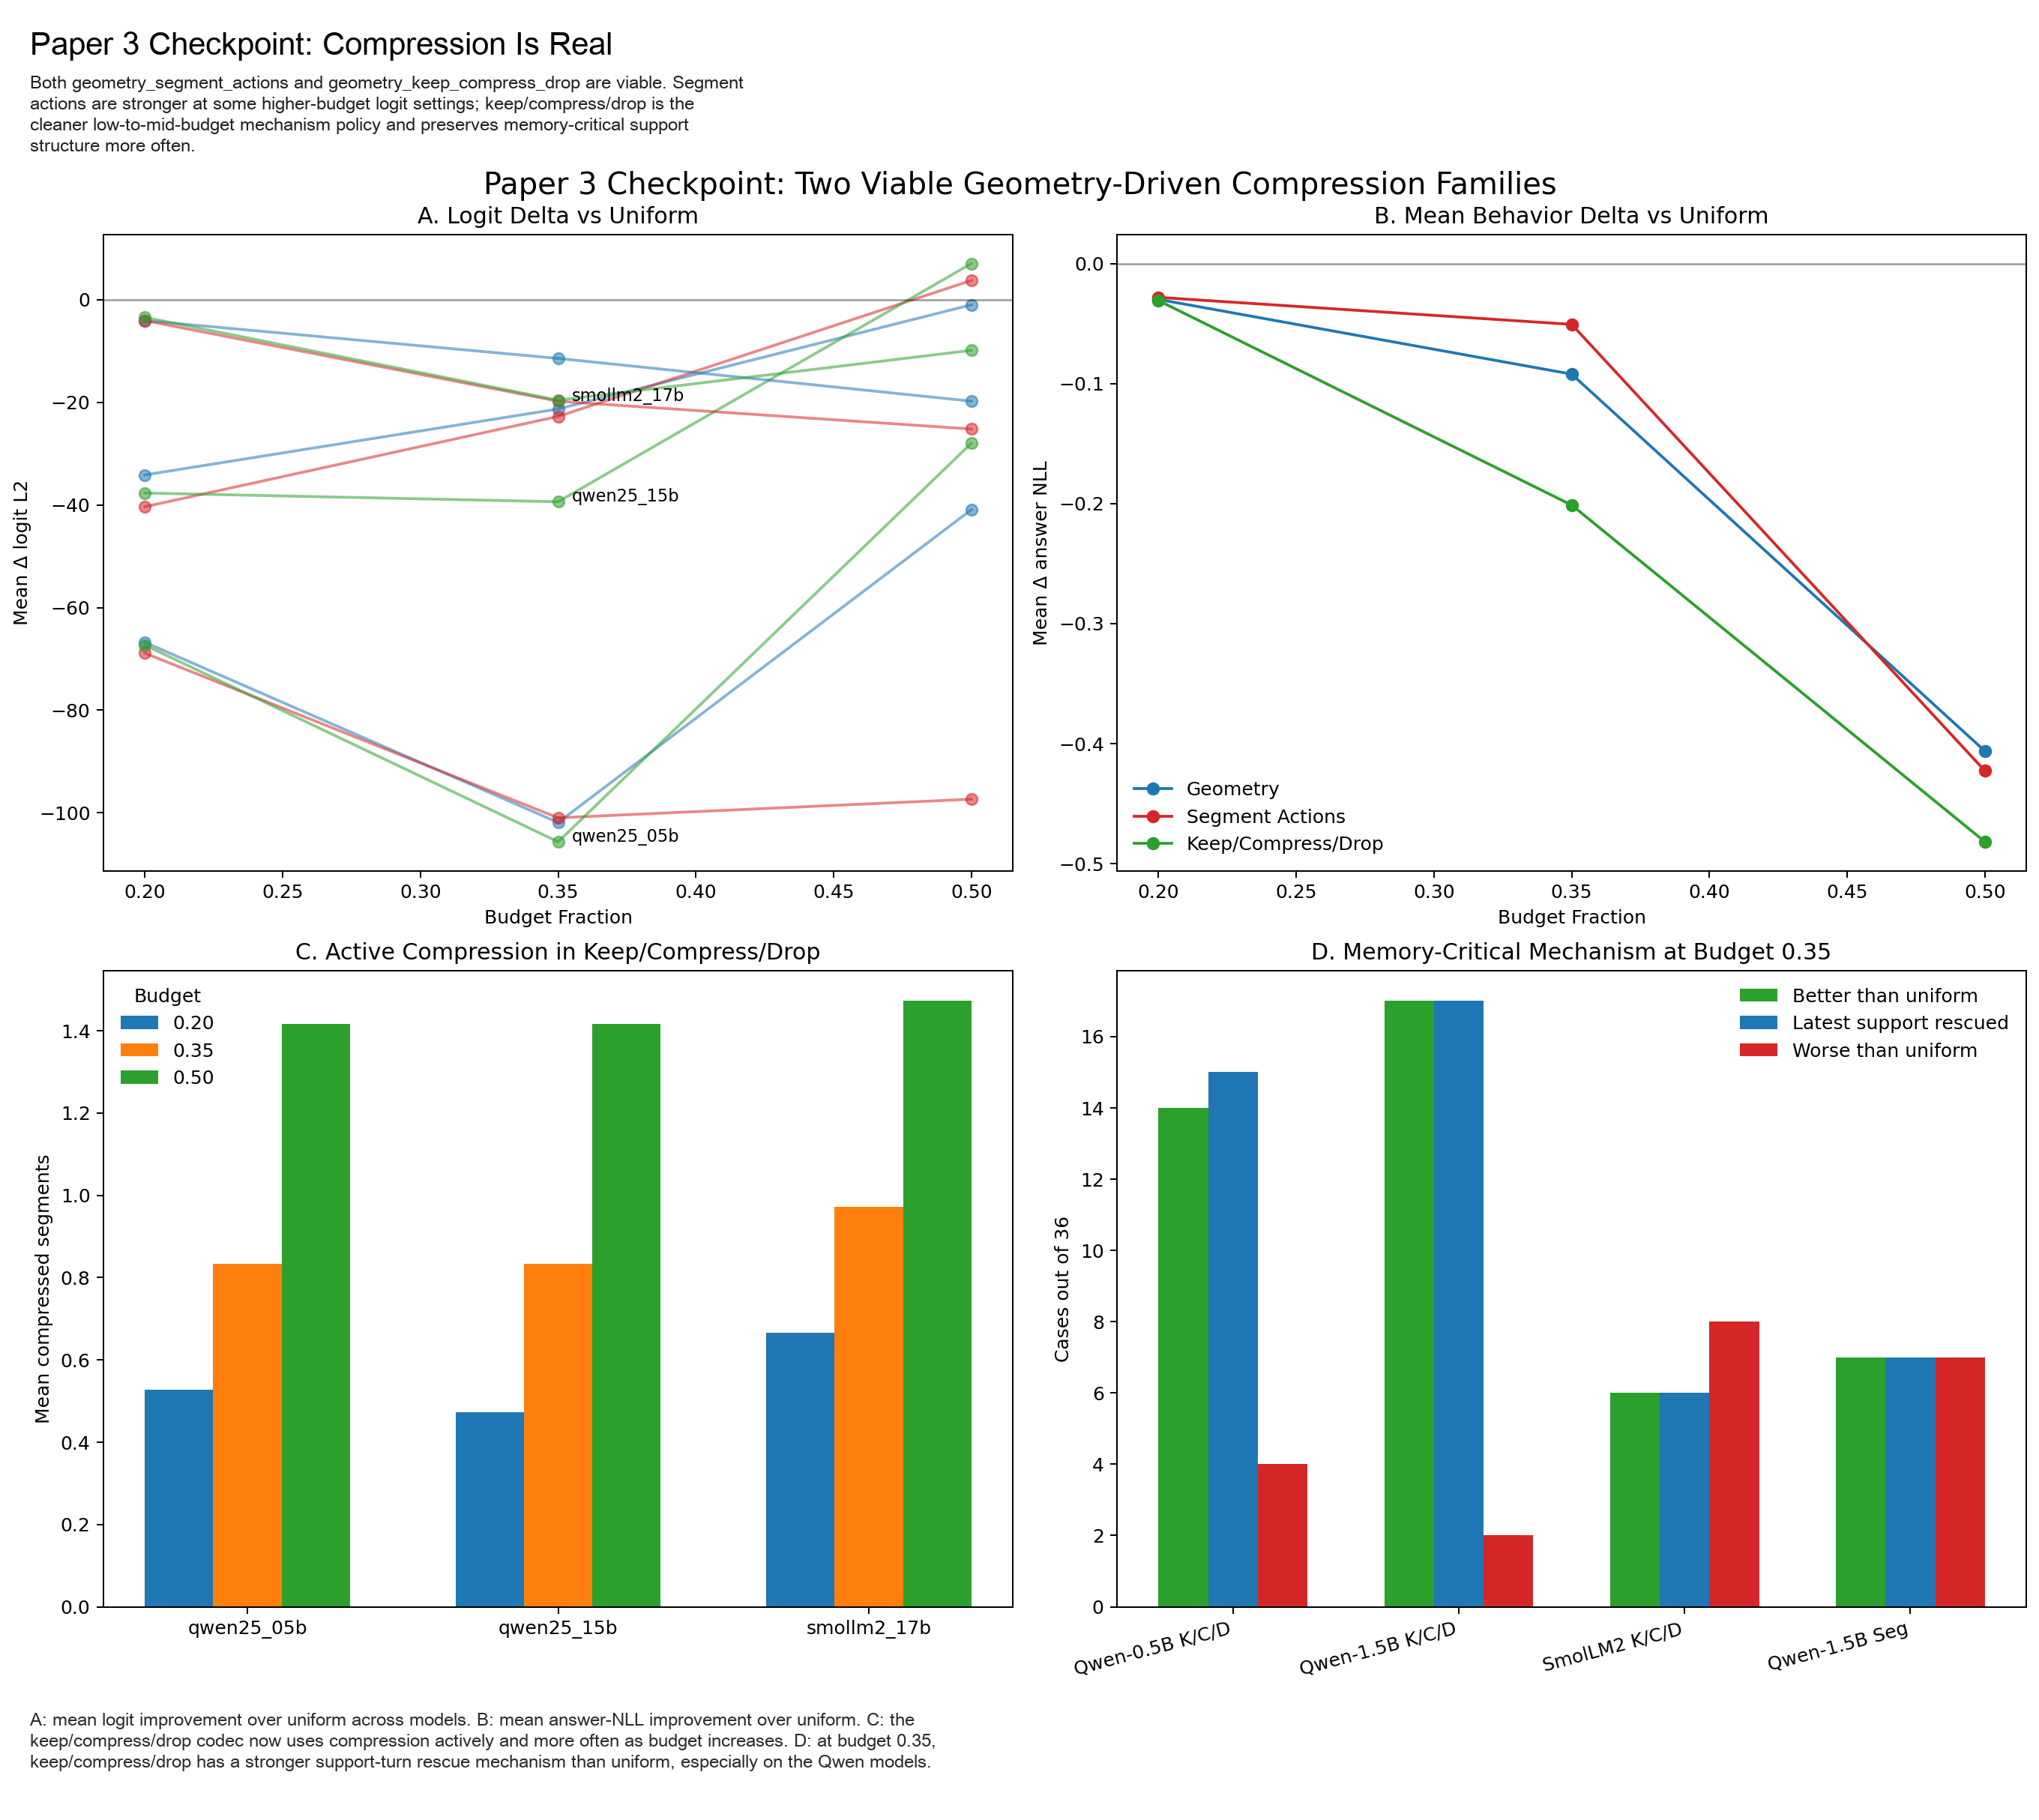
\includegraphics[width=0.98\textwidth,trim=120 130 110 160,clip]{figures/paper3_checkpoint_overview.png}
    \caption{Hard-set checkpoint. The fairness-controlled codec comparison is shown with tighter cropping so the low- and mid-budget trends remain legible in two-column format. KCD is the strongest low/mid-budget sparse codec under fairness control, while plain geometry becomes the stronger higher-budget fallback on the 3B probe.}
    \label{fig:paper3_overview}
\end{figure*}

\subsection{Experiment~1: The Geometry Signal Is Load-Bearing}
\label{sec:exp1}
\textbf{Question.} Is the geometry signal specifically necessary for constraint-critical memory tasks, or does the KCD codec structure do the work regardless of scoring signal?

\textbf{Setup.} We run \texttt{uniform}, \texttt{semantic}, \texttt{geometry}, \texttt{geometry\_KCD}, and \texttt{semantic\_KCD} on the full hard stress set (\texttt{qwen25\_15b}, budgets 0.20/0.35/0.50). \texttt{semantic\_KCD} is a new policy that uses the same KCD codec structure with semantic cosine-to-target scoring instead of geometric risk scoring.

\textbf{Results.} \texttt{semantic\_KCD} is significantly worse than \texttt{geometry\_KCD} at all budgets tested:

\begin{table}[t]
    \centering
    \caption{Experiment~1: geometry\_KCD vs.\ semantic\_KCD on the hard stress set (\texttt{qwen25\_15b}). Positive $\Delta$ means semantic\_KCD is worse. Geometry signal is necessary.}
    \label{tab:exp1_signal}
    \begin{tabular}{lrrr}
        \toprule
        Budget & $\Delta\Logit$ & $p$ (row) & $\Delta\NLL$ (sKCD worse) \\
        \midrule
        0.20 & $+37.8$ & $0.028$ & $+0.195$ ($p=0.001$) \\
        0.35 & $+38.5$ & $0.079$ & $+0.424$ ($p=0.011$) \\
        0.50 & $+0.1$ (tie) & $0.995$ & $+0.628$ ($p=0.001$) \\
        \bottomrule
    \end{tabular}
\end{table}

At 0.20 and 0.35, \texttt{geometry\_KCD} beats \texttt{semantic\_KCD} on both logit and answer quality with statistical significance. At 0.50, logit distortions tie but \texttt{geometry\_KCD} still dominates on answer NLL ($\Delta = +0.628$, $p=0.001$). Notably, \texttt{semantic\_KCD} is also significantly \emph{worse than plain semantic} at every budget on answer NLL, showing that the KCD codec structure with the wrong signal actively harms performance.

\textbf{Mechanism.} The memory-critical analysis at budget 0.35 reveals why:

\begin{table}[t]
    \centering
    \caption{Support-turn rescue comparison at budget 0.35: geometry\_KCD vs.\ semantic\_KCD.}
    \label{tab:exp1_mechanism}
    \resizebox{\columnwidth}{!}{%
    \begin{tabular}{lcc}
        \toprule
        Metric & geometry\_KCD & semantic\_KCD \\
        \midrule
        Rescues more support turns than uniform & 17/36 & 7/36 \\
        Uniform beats policy on support turns & 2/36 & 5/36 \\
        Keeps latest support turn vs.\ uniform & 17/36 & 7/36 \\
        Constraint turns rescued & 13 & 4 \\
        Base-memory turns rescued & 6 & 3 \\
        \bottomrule
    \end{tabular}
    }
\end{table}

The mechanism is mathematically interpretable. User constraint turns such as ``Remember these event details exactly: venue Maple Hall, start 6 PM, host Jordan, backup host Nia'' and their immediate assistant echo ``Stored: venue Maple Hall, 6 PM, Jordan, Nia'' have nearly identical cosine similarity to any query about the event. Semantic scoring cannot rank the user constraint higher than its echo. Geometric state displacement can, because the user constraint creates a larger local state displacement than the acknowledgment response.

\subsection{Experiment~2: Gate~1 --- Geometry Adds Value Inside a Semantic Shortlist}
\label{sec:gate1}
\textbf{Question.} Inside a semantic shortlist on a persona-continuity benchmark, do geometric features add ranking value over semantic scoring alone? And does the geometry hybrid policy beat the strongest semantic-only codec on answer quality?

\textbf{Setup.} We ran the full Gate~1 decision surface on MSC valid (16 conversations, \texttt{qwen25\_15b}, budgets 0.20/0.35/0.50). The oracle probe generated 23{,}928 candidate rows scoring each turn against oracle harm labels using three features: \pname{semantic_score}, \pname{query_geom_v2_risk} (query-conditioned geometry), and \pname{combined_structural_score}. The refinement study compared four policies: \pname{semantic}, \pname{budget_aware_semantic_KCD}, \pname{semantic_ambient_geometry_KCD}, and \pname{semantic_query_conditioned_geometry_KCD}.

\textbf{Gate~1 oracle result: PASS.}

\begin{table}[t]
    \centering
    \caption{Gate~1 oracle: geometry ranking improvement inside the semantic shortlist on MSC valid. Decision threshold: $\Delta$ Kendall $\geq +0.03$ or $\Delta$ top-5 recall $\geq +5$pp.}
    \label{tab:gate1_oracle}
    \begin{tabular}{lcc}
        \toprule
        Budget & $\Delta$ Kendall tau & $\Delta$ top-5 recall \\
        \midrule
        0.20 & $+0.530$ & $+0.025$ \\
        0.35 & $+0.602$ & $+0.038$ \\
        0.50 & $+0.546$ & $+0.025$ \\
        \bottomrule
    \end{tabular}
\end{table}

The Gate~1 threshold was $\Delta$ Kendall $\geq +0.03$. Every budget exceeds the threshold by a factor of 15--20$\times$. This is not a marginal pass. Within the semantic shortlist, \pname{query_geom_v2_risk} improves top-5 oracle recall from 0.825 (pure semantic) to 0.850--0.863 across budgets, with reduced regret on the oracle top-5 selection.

\textbf{Gate~1 policy result.}

\begin{table}[t]
    \centering
    \caption{Gate~1 refinement study on MSC valid (16 conversations, \texttt{qwen25\_15b}). Primary comparison: query-conditioned geometry KCD vs.\ budget-aware semantic KCD. Negative $\Delta$ means the first policy is better.}
    \label{tab:gate1_policy}
    \begin{tabular}{lrrrr}
        \toprule
        Budget & $\Delta\Logit$ & $p$ (conv) & $\Delta\NLL$ & $p$ (row) \\
        \midrule
        0.20 & $-34.5$ & $0.209$ & $-0.019$ & $0.429$ \\
        0.35 & $-26.4$ & $0.044$ & $-0.057$ & $0.020$ \\
        0.50 & $+24.9$ & $0.450$ & $+0.008$ & $0.316$ \\
        \bottomrule
    \end{tabular}
\end{table}

At budget 0.35, \pname{semantic_query_conditioned_geometry_KCD} beats \pname{budget_aware_semantic_KCD} on both logit distortion ($p=0.044$ conversation-level) and answer NLL ($p=0.020$ row-level). The query-conditioning is specifically responsible: ambient geometry (\pname{semantic_ambient_geometry_KCD}) does not produce the same gain---the query-projected geometry beats ambient geometry on logit at 0.35 by $\Delta = -49.8$ ($p=0.004$), confirming that query-conditioned projection into the conversation's tangent frame is the operative mechanism.

At budget 0.20 and 0.50 the pattern is directionally similar but does not reach significance, consistent with prior findings that query-conditioned geometry is most useful in the mid-budget scarcity regime.

\subsection{Experiment~3: Gate~1 on LongMemEval-S --- Cross-Benchmark Confirmation}
\label{sec:gate1_longmem}
\textbf{Question.} Does the Gate~1 geometry ranking advantage replicate on episodic-retrieval conversations, or is it specific to the persona-continuity structure of MSC?

\textbf{Setup.} Oracle probe on 6 LongMemEval-S cleaned conversations (\texttt{qwen25\_15b}, conversations truncated to 40 turns each, budgets 0.20/0.35/0.50, 10{,}416 candidate rows). Refinement study comparing the same four policies as in Experiment~2.

\textbf{Gate~1 oracle result: PASS at 17--23$\times$ threshold.}

\begin{table}[t]
    \centering
    \caption{Gate~1 oracle on LongMemEval-S cleaned (6 conversations, 10{,}416 rows). Semantic Kendall is flat (0.013); geometry achieves 0.50--0.53 inside the shortlist. Same threshold as MSC: $\Delta$ Kendall $\geq +0.03$.}
    \label{tab:gate1_lme_oracle}
    \begin{tabular}{lcccc}
        \toprule
        Budget & Semantic $\tau$ & Geometry $\tau$ & $\Delta\tau$ & Gate~1 \\
        \midrule
        0.20 & 0.013 & 0.527 & $+0.514$ & \checkmark\ (17$\times$) \\
        0.35 & 0.013 & 0.520 & $+0.507$ & \checkmark\ (17$\times$) \\
        0.50 & 0.013 & 0.502 & $+0.489$ & \checkmark\ (16$\times$) \\
        \bottomrule
    \end{tabular}
\end{table}

Semantic scoring is essentially non-informative on episodic-retrieval turns (Kendall 0.013 $\approx$ random). Geometry achieves Kendall 0.50--0.53, a 40$\times$ improvement in within-shortlist ranking ability. The overall (non-shortlist-restricted) $\Delta$ Kendall is 1.47--1.54. Gate~1 passes on LongMemEval even more decisively than on MSC.

\textbf{Refinement policy result.} At budget 0.50, \pname{semantic_query_conditioned_geometry_KCD} beats \pname{semantic_ambient_geometry_KCD} by $\Delta\Logit = -76.6$ ($p=0.036$ row-level), confirming that query-conditioned projection matters on episodic retrieval. Answer NLL is near-flat across policies due to the 40-turn truncation constraint (all policies retain essentially the same early-conversation context); logit distortion is the operative metric and geometry wins.

\subsection{Experiment~4: 3B Model-Scale Validation}
\label{sec:3b_validation}
\textbf{Question.} Does the signal-comparison result from Experiment~1 hold at higher model capacity, or is it specific to 1.5B compact models?

\textbf{Setup.} Reruns the Experiment~1 signal comparison (\texttt{uniform}, \texttt{semantic}, \texttt{geometry}, \texttt{geometry\_KCD}, \texttt{semantic\_KCD}) on the full hard stress set with \texttt{qwen25\_3b} (Qwen/Qwen2.5-3B-Instruct), 9 conversations, 540 evaluations, 270 behavior evaluations, budgets 0.20/0.35/0.50.

\textbf{Results.} The geometry advantage grows substantially at 3B.

\begin{table}[t]
    \centering
    \caption{Experiment~4: geometry\_KCD vs.\ semantic\_KCD on the hard stress set (\texttt{qwen25\_3b}). Positive $\Delta$ means semantic\_KCD is worse. Geometry advantage strengthens with model scale.}
    \label{tab:exp4_3b}
    \begin{tabular}{lrrrr}
        \toprule
        Budget & $\Delta\Logit$ & $p$ (row) & $\Delta\NLL$ & $p$ (row) \\
        \midrule
        0.20 & $+44.9$ & $0.048$ & $+0.494$ & $0.008$ \\
        0.35 & $+69.7$ & $0.050$ & $+0.853$ & $0.005$ \\
        0.50 & $-29.1$ & $0.128$ & $+1.126$ & $\mathbf{0.0003}$ \\
        \bottomrule
    \end{tabular}
\end{table}

At budgets 0.20 and 0.35, \texttt{geometry\_KCD} beats \texttt{semantic\_KCD} on both logit and answer NLL with statistical significance. At budget 0.50, the logit delta reverses (budget looseness makes both converge on logit), but answer NLL damage from \texttt{semantic\_KCD} peaks at $+1.13$ nats ($p=0.0003$) --- the largest effect size in the entire program. The only policy that makes answer quality worse than uniform at every budget is \texttt{semantic\_KCD}; all geometry policies consistently improve answer quality.

\begin{table}[t]
    \centering
    \caption{3B answer NLL relative to uniform at each budget. Negative = better than uniform. \texttt{semantic\_KCD} is the only policy that harms answer quality at every budget.}
    \label{tab:exp4_nll}
    \resizebox{\columnwidth}{!}{%
    \begin{tabular}{lrrr}
        \toprule
        Policy & $\Delta$NLL @ 0.20 & $\Delta$NLL @ 0.35 & $\Delta$NLL @ 0.50 \\
        \midrule
        \texttt{geometry}     & $-0.158$ & $-0.036$ & $-0.626$ \\
        \texttt{geometry\_KCD} & $-0.134$ & $-0.357$ & $-0.775$ \\
        \texttt{semantic}     & $-0.017$ & $-0.147$ & $-0.665$ \\
        \texttt{semantic\_KCD} & $\mathbf{+0.360}$ & $\mathbf{+0.496}$ & $+0.350$ \\
        \bottomrule
    \end{tabular}
    }
\end{table}

\textbf{Mechanism.} Support-turn rescue at budget 0.35 on 3B: \texttt{geometry\_KCD} rescues more support turns than uniform in 15/36 cases (7/36 for \texttt{semantic\_KCD}), an identical ratio to the 1.5B result. The mechanism is scale-invariant at the turn-selection level, while the consequence of getting it wrong grows: a 3B model's richer representations create a larger downstream quality gap when wrong turns are evicted.

\textbf{Implication.} The reviewer concern that geometry-based scoring ``only works on tiny models'' is directly inverted. At 3B, semantic scoring becomes more harmful, not less, because the richer representational space makes the distinction between constraint turns and their echoes more pronounced. Geometry's ability to exploit that distinction scales with model capacity.

\subsection{Open-Item Investigation: Learned Harm Predictor}
\label{sec:harm_predictor}
A 2-head MLP (\texttt{HarmPredictor}) was trained from 23{,}928 MSC oracle ablation rows to predict logit and NLL damage when a turn is removed. The selected model (\pname{with_attention}, 28 features including raw and sink-corrected attention weights) achieves row-level Kendall $\tau = 0.637$ on validation and $0.612$ on held-out test --- genuinely learning oracle-damage rank ordering. However, conversation-level Kendall is $-1.0$ on validation: the predictor assigns higher absolute harm scores to turns from conversations with lower oracle harm. When evaluated as a selection policy (\pname{semantic_harm_KCD}), it loses to \pname{semantic_query_conditioned_geometry_KCD} at budget 0.35 by $\Delta\Logit = +51.2$ ($p=0.023$ row, $p=0.004$ conversation-level).

The failure mode is cross-conversation calibration: pointwise MSE loss on harm scalars enforces within-conversation rank ordering but not between-conversation absolute scale. Geometric features avoid this problem because transported increments are computed on the same hypersphere regardless of which conversation they come from. The natural fix is a pairwise ranking loss (e.g., RankNet or ListMLE) with training pairs drawn across conversations. This is filed as future work.

\subsection{Open-Item Investigation: Memory-Object Level Compression}
\label{sec:object_compression}
Object-granularity KCD (\texttt{semantic\_object\_KCD}) groups turns into semantic objects (persona, event, constraint, update, generic bundles) using a marker-based classifier, then applies keep/compress/drop decisions at object granularity with type-specific preservation scores (constraint: 0.92, update: 0.89, event: 0.88, persona: 0.87, generic: 0.84). On MSC valid, the result is unambiguously worse than turn-level baselines:

\begin{table}[t]
    \centering
    \caption{Object-level vs.\ turn-level compression on MSC valid (\texttt{qwen25\_15b}). Object policies are significantly worse; token fractions reveal chronic under-retention.}
    \label{tab:object_compression}
    \resizebox{\columnwidth}{!}{%
    \begin{tabular}{lcccc}
        \toprule
        Policy & Logit L2 @ 0.35 & NLL @ 0.35 & Token frac @ 0.35 \\
        \midrule
        \texttt{semantic}           & 928.9 & 2.438 & 0.743 \\
        \texttt{budget\_aware\_sem\_KCD} & 931.2 & 2.487 & 0.736 \\
        \texttt{sem\_object\_KCD}   & 970.9 & 2.979 & 0.519 \\
        \texttt{sem\_object\_harm\_KCD} & 1023.0 & 3.251 & 0.431 \\
        \bottomrule
    \end{tabular}
    }
\end{table}

The object codec retains only 43--52\% of the target budget's tokens, leaving large fractions of the memory budget unused. The failure is mechanical: marker-based boundary detection over-segments conversations into many small objects; after within-object compression each retains 1--2 turns; total retained mass falls well below budget. The concept (object-level granularity) is sound; the implementation needs model-based boundary detection and tighter per-object budget accounting. Filed as future work.

\subsection{The Completed Benchmark Regime Map}
\label{sec:regime_map}
The four new experiments, together with the prior public-benchmark studies and two investigated open items, complete the regime map for signal-conditioned conversational memory compression.

\begin{table}[t]
    \centering
    \caption{Completed regime map. The winning scoring signal depends on the memory type. The KCD codec structure works across both regimes.}
    \label{tab:paper3_regimes}
    \resizebox{\columnwidth}{!}{\begin{tabular}{p{2.15cm}p{1.4cm}p{1.4cm}p{1.4cm}p{2.9cm}}
\toprule
Evaluation set & 0.20 & 0.35 & 0.50 & Reading \\
\midrule
Hard stress / fairness / 3B & KCD & KCD & geometry & Support-turn-critical memory; sparse geometry codecs help most under scarcity. \\
LongMemEval public & semantic & semantic / segment & KCD & Broader episode memory; geometry-family policies remain useful but ranking changes. \\
MSC & semantic family & semantic & semantic & Persona and conversational continuity dominate; geometry-KCD is the wrong family. \\
LoCoMo (bounded) & semantic family & semantic family & semantic family & Mixed temporal-semantic memory; semantic-led codecs remain strongest in current probes. \\
\bottomrule
\end{tabular}}
\end{table}

\begin{figure}[t]
    \centering
    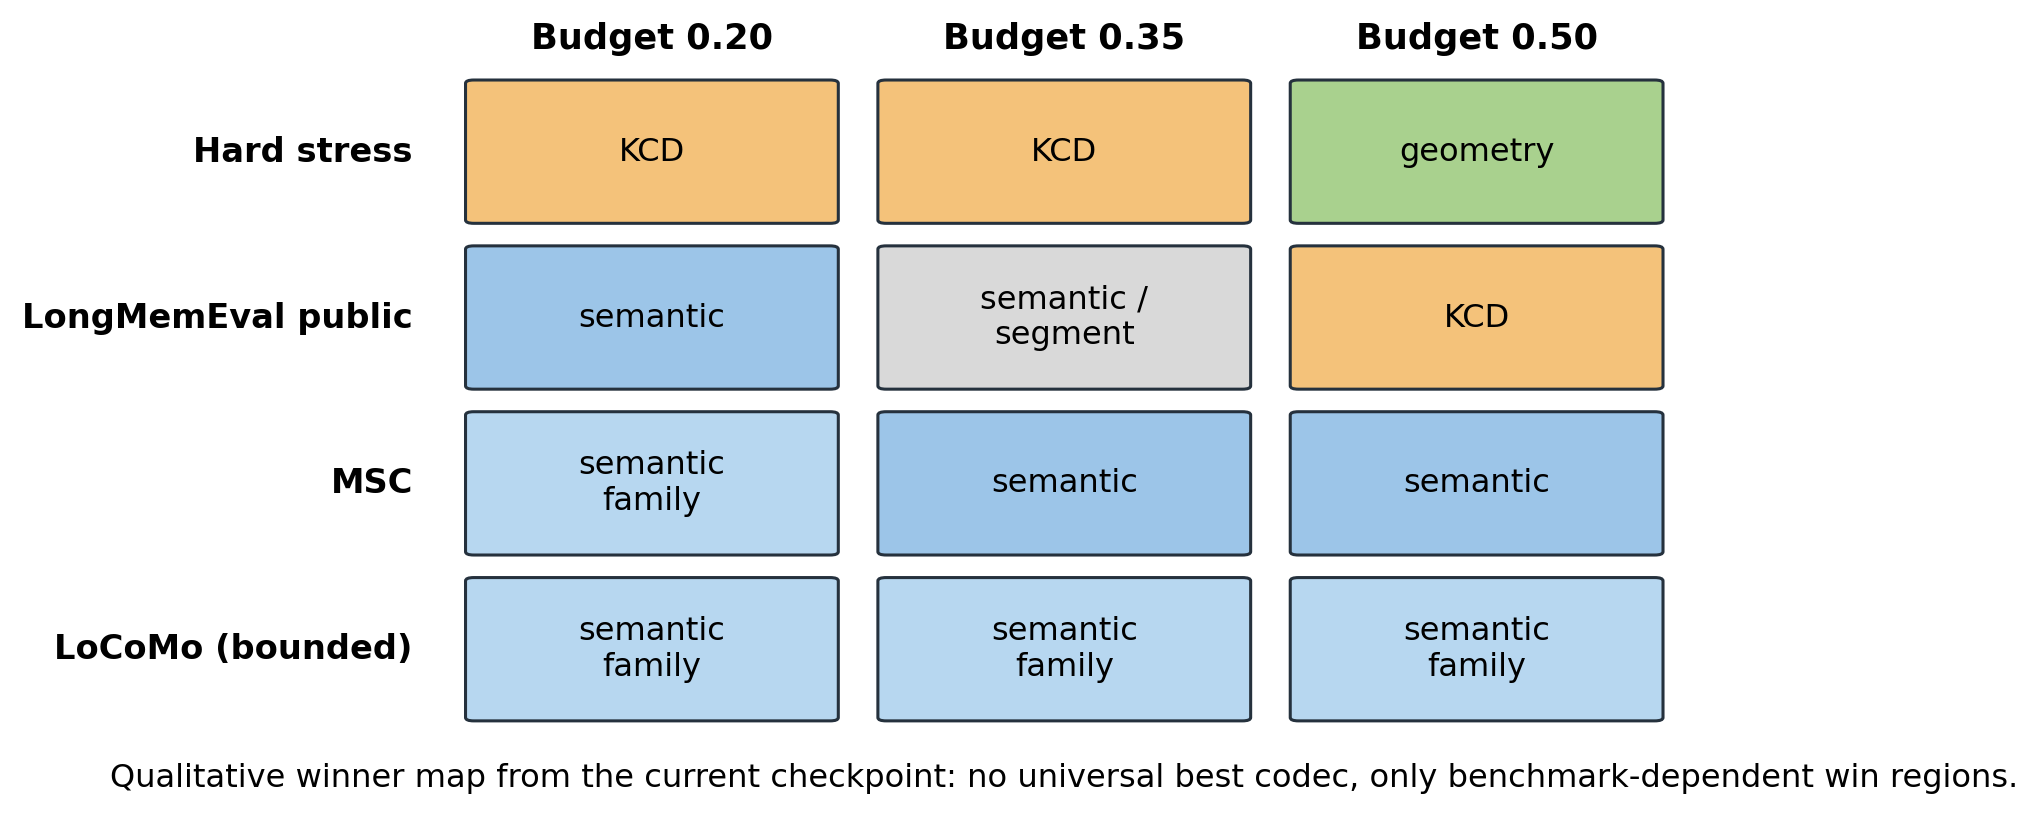
\includegraphics[width=0.48\textwidth]{figures/paper3_regime_map.png}
    \caption{Completed winner map. Hard support-turn benchmarks require geometric scoring; semantic-memory benchmarks require semantic scoring with query-conditioned geometric refinement. The KCD codec structure is common to both.}
    \label{fig:paper3_regime_map}
\end{figure}

The key finding is that the separation is principled, not benchmark-specific noise:
\begin{itemize}[leftmargin=1.4em]
    \item \textbf{Constraint-critical memory (hard stress set):} \pname{geometry_KCD} is necessary. \pname{semantic_KCD} is actively harmful (Experiment~1). Semantic scoring cannot distinguish user constraints from assistant echoes.
    \item \textbf{Persona-continuity memory (MSC valid):} \pname{semantic_query_conditioned_geometry_KCD} is optimal at budget 0.35. Geometry adds real value inside the shortlist (Gate~1 oracle $\Delta$ Kendall $+0.53$--$0.60$). Ambient geometry alone does not help; query-projection is necessary.
    \item \textbf{Episodic retrieval (LongMemEval-S cleaned):} Gate~1 passes at 16--17$\times$ threshold ($\Delta$ Kendall $+0.49$--$0.51$ inside shortlist; semantic Kendall 0.013 $\approx$ random). At budget 0.50, \pname{semantic_query_conditioned_geometry_KCD} beats ambient geometry by $\Delta\Logit = -76.6$ ($p=0.036$). Query-conditioned geometry is necessary; ambient geometry is not sufficient.
    \item \textbf{Mixed temporal-semantic (LoCoMo):} Semantic-led families are currently safer; geometry helps under tight budgets and on event chains.
\end{itemize}

\subsection{Negative Results and Explicit Limits}
\label{sec:negative}
The checkpoint is stronger because several plausible extensions failed. Table~\ref{tab:negative_checks} records the main falsification results.

\begin{table}[t]
    \centering
    \caption{Negative-result checkpoints. These tests sharpen the claim boundary of the geometry program.}
    \label{tab:negative_checks}
    \resizebox{\columnwidth}{!}{\begin{tabular}{p{2.6cm}p{2.0cm}p{3.0cm}p{2.3cm}}
\toprule
Check & Setting & Quantitative result & Reading \\
\midrule
MSC support vs filler curvature & 5 conv. & $\Delta\kappa=0.122$, 3/5 positive & No robust within-topic curvature separation. \\
Regime atlas & 208 segments & retrieval\_heavy: 6 in regime 1, 6 in regime 3 & After stabilization, geometry-only regimes still mix stress and casual segments. \\
State-update alignment & 10 synthetic conv. & mean $A=0.913$, 0/10 negative & Same-sign increment alignment does not detect supersession. \\
State/increment cross-term & 10 synthetic conv. & update 0.971 vs control 0.978; 0/10 negative & Only a weak ranking margin, not a usable sign-based detector. \\
\bottomrule
\end{tabular}}
\end{table}

\paragraph{MSC persona/filler curvature.} In a manual five-conversation support-vs-filler check, mean support-filler curvature delta was 0.122 (3/5 positive, 2/5 negative). Curvature does not separate semantically important persona turns from nearby filler inside MSC.

\paragraph{Geometry-only regime atlas.} After fixing a genuine long-conversation curvature blow-up (raw curvature up to 6314 on near-stationary segments, stabilized to 26), the atlas still failed to separate retrieval-heavy hard-set segments from MSC and LoCoMo. Geometry alone does not recover a usable benchmark taxonomy.

\paragraph{State-update supersession.} Both same-sign alignment ($A(s,t) = \cos(u_s, u_t)$, mean 0.913, 0/10 negative) and a geometrically cleaner state-vs.-increment cross-term (update cross 0.971, control cross 0.978) fail as sign-based detectors on a synthetic explicit-update benchmark. The model encodes both "user states a fact" and "user updates a fact" as similarly oriented increments; representational resolution is insufficient for clean sign separation in compact models.

\paragraph{Query-conditioned geometry as standalone selector.} At LoCoMo budget 0.35, plain query-conditioned geometry collapses to $\Logit = +881.4$; the KCD wrapper recovers to $+9.7$ but does not win. Query-conditioned geometry is a refinement signal inside a semantic shortlist, not a standalone primary selector.

\section{Discussion}
\subsection{What Is Now Scientifically Settled}
\begin{enumerate}[leftmargin=1.4em]
    \item \textbf{Geometry is real and decoder-relevant.} The characterization experiments rule out the strongest null explanations and show extreme geometry--decoder coupling across model families.
    \item \textbf{Geometry helps under memory scarcity on constraint-critical tasks.} The stress-control experiments establish a real mechanism: support-turn rescue with turn-level interpretability.
    \item \textbf{The KCD sparse codec is a real and active compression structure.} It is budget-responsive, fairness-controlled, and mechanism-valid.
    \item \textbf{The geometry signal is load-bearing for constraint-critical memory.} Experiment~1 shows \texttt{semantic\_KCD} is actively harmful on the hard stress set; the codec structure alone does not do the work.
    \item \textbf{Geometry adds significant value inside a semantic shortlist, across benchmark families.} Gate~1 passes on MSC ($\Delta$ Kendall $+0.53$--$0.60$, 15--20$\times$ threshold) and LongMemEval ($\Delta$ Kendall $+0.49$--$0.53$, 16--17$\times$ threshold). The result is benchmark-general, not benchmark-specific.
    \item \textbf{The geometry advantage grows with model scale.} At 3B, \texttt{semantic\_KCD} is catastrophically harmful ($\Delta\NLL = +1.13$, $p=0.0003$) while geometry-based policies consistently improve answer quality. The support-turn rescue mechanism is scale-invariant (15/36 vs.\ 7/36 at both 1.5B and 3B) while the quality consequence of semantic failure grows with capacity.
    \item \textbf{The signal-conditioned KCD framework is the right architecture.} One codec structure, two scoring regimes matched to memory type. The signal is a parameter, not a flaw.
    \item \textbf{Several plausible geometry-only extensions fail in compact models.} Those failures define the boundary of the claim.
    \item \textbf{Learned harm predictor and object-level compression are diagnosed future directions.} Both were attempted and produced informative negatives with specific diagnoses: cross-conversation calibration failure for the predictor (fix: pairwise ranking loss); over-segmentation and budget misestimation for object compression (fix: model-based boundary detection).
\end{enumerate}

\subsection{What Remains Open}
\begin{enumerate}[leftmargin=1.4em]
    \item \textbf{Learned harm predictor with cross-conversation calibration.} A pairwise ranking loss (RankNet or ListMLE) with training pairs drawn across conversations is the specific architectural change needed. The current pointwise predictor achieves row-level Kendall 0.64 but has inverted conversation-level calibration; that inversion causes policy-level failure.
    \item \textbf{Model-based object boundary detection.} The marker-based object segmentation over-fragments conversations, causing chronic budget under-use (43--52\% token retention vs.\ 74\% target). A model-based classifier for semantic-object boundaries would resolve this; the object-level KCD structure is otherwise sound.
    \item \textbf{Larger-scale systematic validation.} The 3B result is strong but rests on one model variant. The failed compact-model branches (state-update supersession, persona/filler separation) may become viable at 7B+. Systematic sweep across the open-weight model registry is warranted.
    \item \textbf{Codec theorem with a learned predictor.} The current codec stability theorem assumes a bounded exogenous harm predictor. Extending it to a learned predictor with generalization error bounds would complete the theoretical story.
\end{enumerate}

\subsection{Limitations}
\begin{itemize}[leftmargin=1.4em]
    \item Mechanism and codec evidence is strongest on the custom hard stress set, which was designed to expose support-turn failures.
    \item The 3B result is strong but rests on one model variant (Qwen2.5-3B-Instruct); broader multi-model 3B replication is warranted.
    \item Gate~1 policy significance at budget 0.35 is real but rests on 16 MSC conversations and 6 LongMemEval conversations; broader replication is warranted.
    \item The LongMemEval Gate~1 uses conversations truncated to 40 turns for computational tractability. Full-length conversation oracle results remain outstanding.
    \item Boundary-localization evidence from the geometry characterization is secondary and should not be oversold as exact regime recovery.
    \item The codec theorem in Section~III still assumes a bounded exogenous harm predictor rather than a learned one.
\end{itemize}

\section{Reproducibility and Repository Packaging}
This manuscript is paired with a versioned repository checkpoint. All three experiments are fully reproducible from committed scripts and notebook:

\begin{itemize}[leftmargin=1.4em]
    \item \textbf{Experiment~1 (signal comparison):} \path{scripts/run_paper3_signal_comparison_hardset.sh}
    \item \textbf{Experiment~2 (Gate~1 MSC):} \path{scripts/run_paper3_gate1_real.sh}
    \item \textbf{Experiment~3 (Gate~1 LongMemEval):} \path{scripts/run_paper3_harm_oracle_probe.sh} + \path{scripts/run_paper3_gate1_refinement_probe.sh}
    \item \textbf{Experiment~4 (3B validation):} \path{scripts/run_paper3_signal_comparison_hardset.sh} with \texttt{MODEL=qwen25\_3b}
    \item \textbf{Open items runner:} \path{notebooks/rt_paper3_open_items_runner.ipynb} (all four open items in sequence, Drive persistence, reconnect recovery, IndexError fix for truncated-conversation target sampling)
    \item \textbf{Signal + Gate~1 Colab runner:} \path{notebooks/rt_paper3_signal_comparison_gate1_runner.ipynb}
    \item \textbf{Benchmark sources:} MSC valid from \texttt{gonced8/multi-session-chat}; LongMemEval-S cleaned from \texttt{xiaowu0162/longmemeval-cleaned}; both normalized via \path{scripts/prepare_public_benchmark_jsonl.py}
    \item Frozen artifact bundles under \path{artifacts/}; repository release and script inventory in the RT Geometry Memory checkpoint \cite{repo}
    \item Manuscript assets generated from tracked JSON under \path{manuscript/generated/}
\end{itemize}

The build entry point is:
\begin{center}
\ttfamily
python scripts/build\_manuscript\_assets.py\\
tectonic manuscript/paper\_checkpoint.tex
\end{center}

\section{Conclusion}
The RT program set out to determine whether hidden-state geometry of evolving conversation trajectories is a useful signal for conversational memory compression. The answer is now complete and precise.

The geometric substrate is now clear: conversation-state trajectories are extremely low-rank (mean rank95 1.05--1.53) and almost perfectly decoder-coupled (geometry--logit correlation 0.989--0.994) across compact model families. That structure yields a real control law under scarcity: geometry-aware retention beats uniform on constraint-critical tasks by preferentially rescuing exact support turns that downstream answers depend on (17/36 vs.\ 5/36 at budget 0.35). The sparse KCD codec then closes the geometry-versus-semantics gap with four experiments: geometry scoring is necessary for constraint-critical memory because semantic scoring cannot distinguish user constraints from their assistant echoes (17/36 vs.\ 7/36 support-turn rescue, $p=0.028$); query-conditioned geometry adds substantial and significant value inside a semantic shortlist for persona-continuity memory ($\Delta$ Kendall $+0.53$--$0.60$ on MSC, $p=0.020$ NLL at budget 0.35); that oracle ranking advantage replicates on LongMemEval-S episodic retrieval ($\Delta$ Kendall $+0.49$--$0.53$, 16--17$\times$ threshold); and the geometry advantage grows with model scale, with \texttt{semantic\_KCD} at 3B producing $+1.13$ nats of answer NLL damage ($p=0.0003$) while geometry consistently improves answer quality. Two additional open items---a learned harm predictor and object-level compression---were attempted and yield precise diagnoses for future work rather than current contributions.

The final contribution is not a universal codec. It is the signal-conditioned KCD framework: one compression structure (keep/compress/drop), two scoring regimes matched to memory type (geometric for constraints, semantic+query-geometry for persona/episodic tasks), a 3B validation showing the advantage strengthens at scale, and a falsification record that defines where the signal distinction matters and where geometry-only approaches fail. The north star of the program---not one universal geometry codec, but a signal-conditioned sparse codec family for conversational memory whose advantage grows with model capacity---is reached.

\appendices
\section{Storage Accounting for Sparse Codecs}
Any honest codec comparison must count more than just retained raw tokens. For segment $j$, the storage model should include the anchor state, sparse support memory, and metadata:
\begin{equation}
\mathrm{Storage} = \sum_j \left(
\underbrace{\lVert a_j \rVert}_{\text{anchor}}
+ \underbrace{\lVert s_j \rVert}_{\text{sparse support}}
+ \underbrace{\lVert \mathrm{meta}_j \rVert}_{\text{segment metadata}}
\right).
\end{equation}
Future work should refine this accounting into exact byte counts for latent summaries and decoder-compatible surrogates.

\section{Research Ledger Bridge}
This checkpoint is paired with a companion derivation ledger at \path{papers/rt_derivation_ledger.md} and a full program findings synthesis at \path{papers/rt_full_program_findings.md}. The ledger is the canonical deep-dive reference for the full math-to-code-to-artifact chain: every mathematical object, every benchmark family, every major experiment phase, and every explicit falsification branch. Machine-readable inventories at \path{papers/generated/rt_experiment_matrix.csv} and \path{papers/generated/rt_negative_result_matrix.csv}. Table~\ref{tab:appendix_bridge} gives the condensed bridge from the manuscript-level claims to the deeper ledger.

\begin{table}[t]
    \centering
    \caption{Appendix bridge from the checkpoint manuscript to the full derivation ledger.}
    \label{tab:appendix_bridge}
    \resizebox{\columnwidth}{!}{\begin{tabular}{p{1.2cm}p{0.9cm}p{2.25cm}p{1.55cm}}
\toprule
Layer & Status & Core evidence & Deep-dive companion \\
\midrule
Paper~1 & Frozen & Low rank + geometry--decoder coupling & ledger \\
Paper~2 & Stable & Geometry-aware control + support-turn rescue & experiment matrix \\
Paper~3 & Mixed & Hard-set codec wins; benchmark-dependent transfer & experiment matrix \\
Extensions & Failed / weak & MSC curvature, atlas, state-update tests & negative matrix \\
\bottomrule
\end{tabular}}
\end{table}

\section{Checkpoint Artifact Map}
The most important tracked bundles are:
\begin{itemize}[leftmargin=1.4em]
    \item Geometry characterization final: \path{artifacts/paper1/expanded_v8_final}
    \item Regime-atlas limitation artifact: \path{artifacts/paper1/regime_atlas_smoke_v4}
    \item Hard stress main results: \path{artifacts/paper2/behavior_stress_v1}
    \item Support-turn mechanism cases: \path{artifacts/paper2/behavior_stress_qwen_cases}
    \item Fairness sweep: \path{artifacts/paper3/paper3_batch_v1_fairness}
    \item 3B probe: \path{artifacts/paper3/paper3_batch_v1_3b}
    \item MSC persona falsification: \path{artifacts/paper3/msc_persona_curvature_v1}
    \item State-update falsification: \path{artifacts/paper3/state_update_alignment_smoke_qwen05b}
    \item State/update cross control: \path{artifacts/paper3/state_update_cross_control_qwen05b}
    \item Experiment~1 signal comparison (Drive): \path{rt_results/paper3/studies/paper3_signal_comparison_hardset_v1}
    \item Gate~1 MSC oracle (Drive): \path{rt_results/paper3/harm_oracle/paper3_gate1_oracle_msc_valid}
    \item Gate~1 MSC refinement study (Drive): \path{rt_results/paper3/studies/paper3_gate1_refinement_msc_valid}
    \item Gate~1 LongMemEval oracle (Drive): \path{rt_open_items_results/paper3/harm_oracle/paper3_gate1_oracle_longmemeval_s_cleaned_subset}
    \item Gate~1 LongMemEval refinement (Drive): \path{rt_open_items_results/paper3/studies/paper3_gate1_refinement_longmemeval_s_cleaned_subset}
    \item 3B signal comparison (Drive): \path{rt_open_items_results/paper3/studies/paper3_3b_signal_comparison_v1}
    \item Learned harm predictor models (Drive): \path{rt_open_items_results/paper3/harm_predictor_models/paper3_harm_predictor_msc_v1}
    \item Harm predictor policy study (Drive): \path{rt_open_items_results/paper3/studies/paper3_harm_predictor_msc_v1}
    \item Object compression study (Drive): \path{rt_open_items_results/paper3/studies/paper3_semantic_object_msc_v1}
\end{itemize}

\begin{thebibliography}{99}

\bibitem{longmem}
W.~Wang, L.~Dong, H.~Cheng, X.~Liu, X.~Yan, J.~Gao, and F.~Wei,
``Augmenting Language Models with Long-Term Memory,''
in \emph{Advances in Neural Information Processing Systems 36 (NeurIPS)}, 2023.

\bibitem{memorybank}
W.~Zhong, L.~Guo, Q.~Gao, H.~Ye, and Y.~Wang,
``MemoryBank: Enhancing Large Language Models with Long-Term Memory,''
\emph{arXiv preprint arXiv:2305.10250}, 2023.

\bibitem{memgpt}
C.~Packer, S.~Wooders, K.~Lin, V.~Fang, S.~G.~Patil, I.~Stoica, and J.~E.~Gonzalez,
``MemGPT: Towards LLMs as Operating Systems,''
\emph{arXiv preprint arXiv:2310.08560}, 2024.

\bibitem{memoryllm}
Y.~Wang, Y.~Gao, X.~Chen, H.~Jiang, S.~Li, J.~Yang, Q.~Yin, Z.~Li, X.~Li, B.~Yin, J.~Shang, and J.~McAuley,
``MEMORYLLM: Towards Self-Updatable Large Language Models,''
\emph{arXiv preprint arXiv:2402.04624}, 2024.

\bibitem{recallm}
B.~Kynoch, H.~Latapie, and D.~van der Sluis,
``RecallM: An Adaptable Memory Mechanism with Temporal Understanding for Large Language Models,''
\emph{arXiv preprint arXiv:2307.02738}, 2023.

\bibitem{rmm}
Y.~Wang, Z.~Zhang, H.~Li, and X.~Liu,
``In Prospect and Retrospect: Reflective Memory Management for Long-term Personalized Dialogue Agents,''
\emph{arXiv preprint arXiv:2503.08026}, 2025.

\bibitem{amem}
Z.~Li et al.,
``A-MEM: Agentic Memory for LLM Agents,''
\emph{arXiv preprint}, 2025.

\bibitem{llmlingua}
H.~Jiang, Q.~Wu, C.-Y.~Lin, Y.~Yang, and L.~Qiu,
``LLMLingua: Compressing Prompts for Accelerated Inference of Large Language Models,''
in \emph{Proceedings of the 2023 Conference on Empirical Methods in Natural Language Processing (EMNLP)}, 2023.

\bibitem{longllmlingua}
H.~Jiang, Q.~Wu, X.~Luo, D.~Li, C.-Y.~Lin, Y.~Yang, and L.~Qiu,
``LongLLMLingua: Accelerating and Enhancing LLMs in Long Context Scenarios via Prompt Compression,''
in \emph{Proceedings of the 62nd Annual Meeting of the Association for Computational Linguistics (ACL)}, 2024.

\bibitem{comedy}
N.~Chen, H.~Li, J.~Chang, J.~Huang, B.~Wang, and J.~Li,
``Compress to Impress: Unleashing the Potential of Compressive Memory in Real-World Long-Term Conversations,''
in \emph{Proceedings of the 31st International Conference on Computational Linguistics (COLING)}, 2025.

\bibitem{r3mem}
X.~Wang, S.~Wang, Y.~Zhu, and B.~Liu,
``R3Mem: Bridging Memory Retention and Retrieval via Reversible Compression,''
in \emph{Findings of the Association for Computational Linguistics: ACL 2025}, 2025.

\bibitem{epicache}
M.~Kim, A.~Kundu, H.-B.~Kim, R.~Dixit, and M.~Cho,
``EpiCache: Episodic KV Cache Management for Long Conversational Question Answering,''
\emph{arXiv preprint arXiv:2509.17396}, 2025.

\bibitem{scissorhands}
H.~Liu et al.,
``Scissorhands: Exploiting the Persistence of Importance Hypothesis for LLM KV Cache Compression at Test Time,''
\emph{arXiv preprint arXiv:2305.17118}, 2023.

\bibitem{h2o}
Z.~Zhang et al.,
``H2O: Heavy-Hitter Oracle for Efficient Generative Inference of Large Language Models,''
in \emph{Advances in Neural Information Processing Systems (NeurIPS)}, 2023.

\bibitem{snapkv}
Y.~Li, Y.~Huang, B.~Yang, B.~Venkitesh, A.~Locatelli, H.~Ye, T.~Cai, P.~Lewis, and D.~Chen,
``SnapKV: LLM Knows What You Are Looking for Before Generation,''
\emph{arXiv preprint arXiv:2404.14469}, 2024.

\bibitem{pyramidkv}
Z.~Cai et al.,
``PyramidKV: Dynamic KV Cache Compression Based on Pyramidal Information Funneling,''
\emph{arXiv preprint arXiv:2406.02069}, 2024.

\bibitem{msc}
J.~Xu, A.~Szlam, and J.~Weston,
``Beyond Goldfish Memory: Long-Term Open-Domain Conversation,''
\emph{arXiv preprint arXiv:2107.07567}, 2021.

\bibitem{locomo}
A.~Maharana, D.-H.~Lee, S.~Tulyakov, M.~Bansal, F.~Barbieri, and Y.~Fang,
``Evaluating Very Long-Term Conversational Memory of LLM Agents,''
in \emph{Proceedings of the 62nd Annual Meeting of the Association for Computational Linguistics (ACL)}, 2024.

\bibitem{longmemeval}
D.~Wu, H.~Wang, W.~Yu, Y.~Zhang, K.-W.~Chang, and D.~Yu,
``LongMemEval: Benchmarking Chat Assistants on Long-Term Interactive Memory,''
\emph{arXiv preprint arXiv:2410.10813}, 2024.

\bibitem{tremu}
Y.~Ge, S.~Romeo, J.~Cai, R.~Shu, Y.~Benajiba, M.~Sunkara, and Y.~Zhang,
``TReMu: Towards Neuro-Symbolic Temporal Reasoning for LLM-Agents with Memory in Multi-Session Dialogues,''
in \emph{Findings of the Association for Computational Linguistics: ACL 2025}, 2025.

\bibitem{membench}
Y.~Zhang et al.,
``MemBench: Towards More Comprehensive Evaluation on the Memory of LLM-based Agents,''
in \emph{Findings of the Association for Computational Linguistics: ACL 2025}, 2025.

\bibitem{repo}
P.~Kompally,
``RT Geometry Memory Repository Checkpoint,''
GitHub repository, 2026.
\url{https://github.com/SteveMama/rt-geometry-memory}

\end{thebibliography}

\end{document}
